\textbf{Definitions, Notations, and Conventions}

Always assume surface $\Sigma$ (our case $\Sigma = \torus$) is oriented.

define cellular decomp of surface

$V,E,F$ are set of vertices, edges, faces.
No bigon faces.

$\vec{E}$ is the set of oriented edges.
We may identify an oriented edge $\vec{e}$ with the pair $(f_{\vec{e}}, e)$,
where $f_{\vec{e}}$ is the face to the left of $\vec{e}$.

When we use $\cev{e}$ to refer to an oriented edge, it refers to
the oppositely oriented edge to $\vec{e}$.
If we construct an expression with both $\vec{e}$ and $\cev{e}$,
it will always be (anti-)symmetrical in the two orientations,
and we assume that an arbitrary choice has been made.

%===============================================================================


Recall circle pattern.

A circle pattern is determined by the radius of the circle $C_f$ associated to each face, $r_f$,
and the angle that each edge subtends in adjacent faces, $\vphi_{\vec{e}}$.
(See \figref{f:circle_pattern})
\begin{figure}
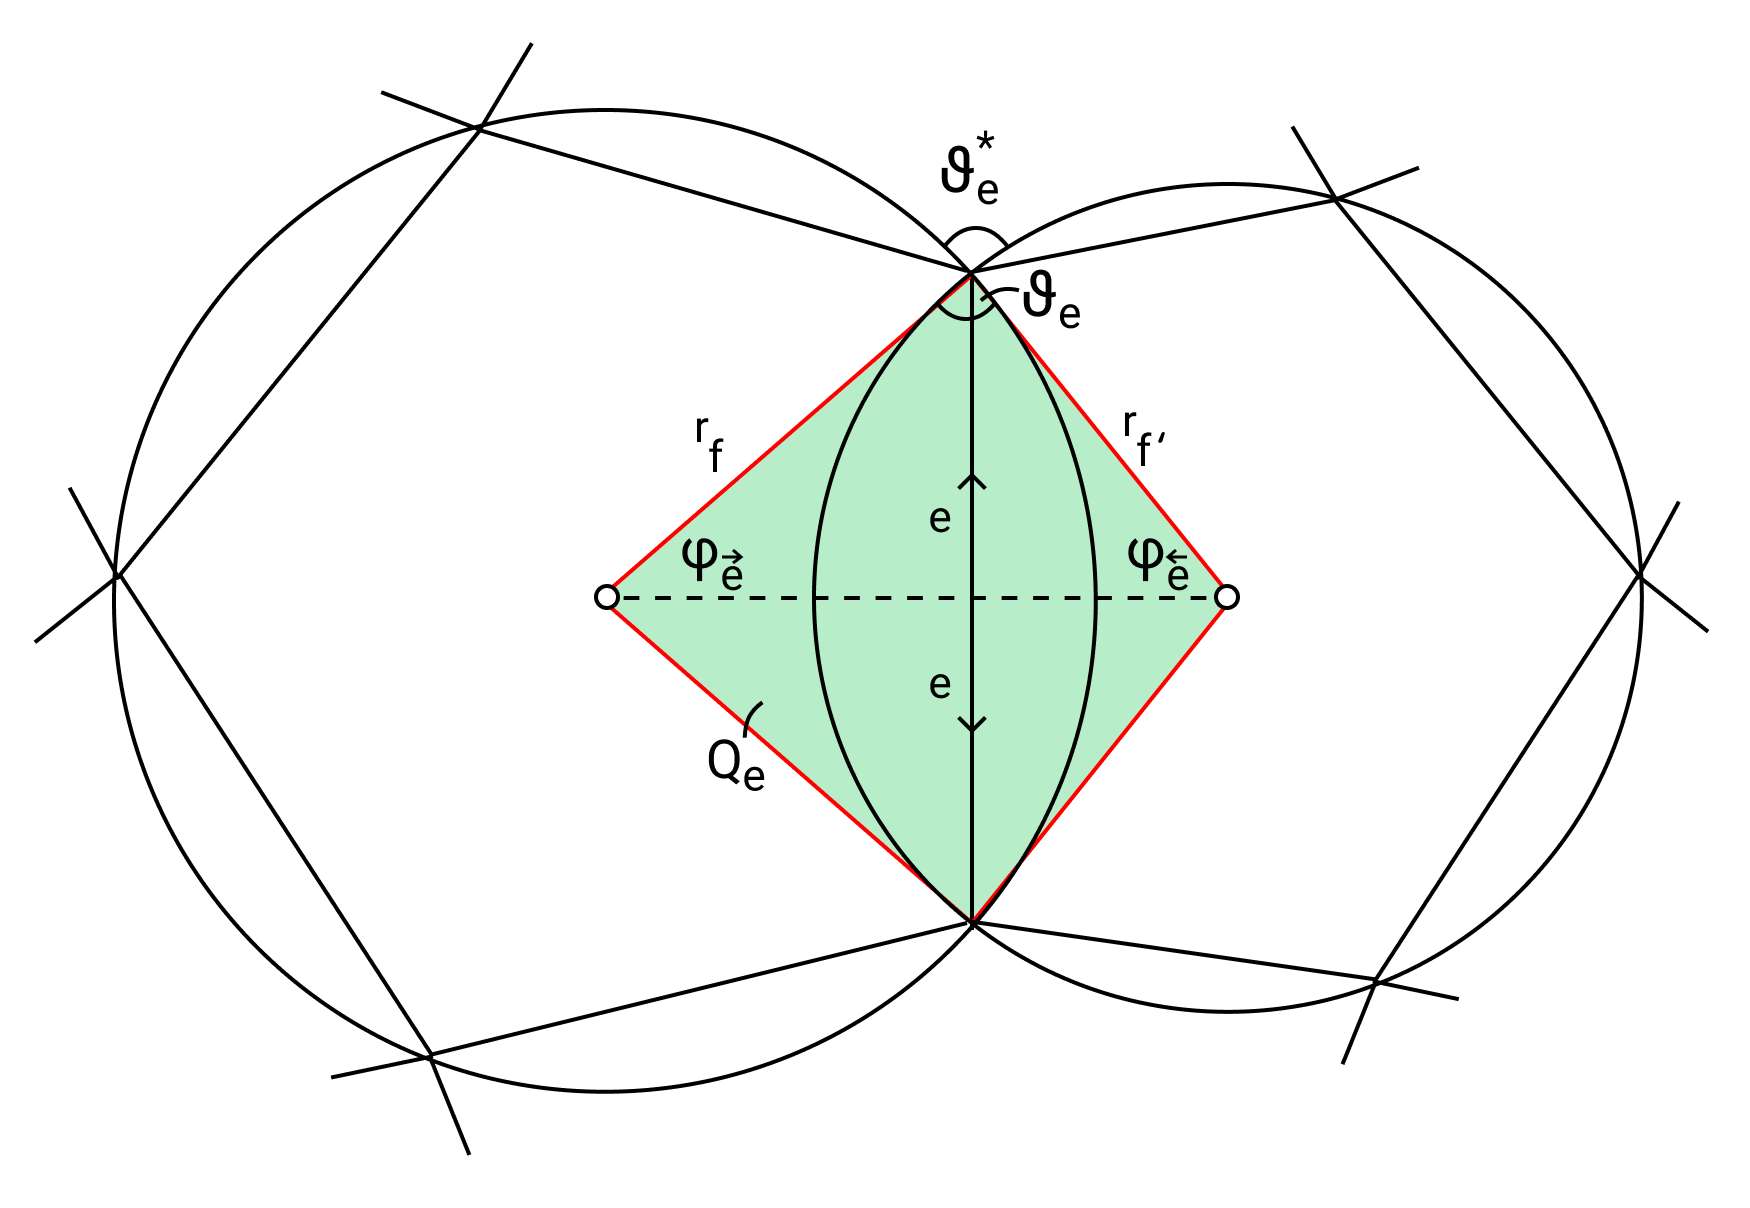
\includegraphics[width=5cm]{circle_pattern}
\caption{Circle pattern in terms of radii $r_f$ and angles $\vphi_{\vec{e}}$}
\label{f:circle_pattern}
\end{figure}
Thus determines, and is determined by a point in $\RRR \times \QQQ$, where

\begin{itemize}
	\item $\RRR := \RR_+^F = \{(r_f)_{f\in F} | r_f \in \RR_+\}$
	\item $\QQQ := \RR^{\vec{E}} =
		\{(\vphi_{\vec{e}})_{\vec{e} \in \vec{E}} | \vphi_{\vec{e}} \in \RR\}$
\end{itemize}
but clearly not every point $c\in \RRR \times \QQQ$ determines a circle pattern.


On $\RRR \times \QQQ$, there are several functions to consider:
\begin{itemize}
	\item $\Phi_f = 2 \sum_{\vec{e} \in \del f} \vphi_{\vec{e}}$, measuring the cone angle
		at the center of $C_f$
	\item $\theta_e = \pi - \vphi_{\vec{e}} - \vphi_{\cev{e}}$
	\item $l_{\vec{e}} = 2 r_{f_{\vec{e}}} \sin \vphi_{\vec{e}}$
\end{itemize}

These fit together to give maps to the following spaces:

\begin{itemize}
	\item $\PPP := \RR^F = \{(\Phi_f)_{f\in F} | \Phi_f \in \RR\}$
	\item $\TTT := \RR^E = \{(\theta_e)_{e \in E} | \theta_e \in \RR\}$
	\item $\LLL := \RR^{\vec{E}} = \{(l_{\vec{e}})_{\vec{e} \in E} | l_{\vec{e}} \in \RR\}$
\end{itemize}


Our main argument is to deform ``degenerate" circle patterns,
where adjacent circles may
be identical or tangent, into ones that don't look so degenerate,
hence it is conveneint to extend the notion of circle pattern:

\begin{definition}
Let $\Gamma$ be a graph on the torus.
An \emph{extended circle pattern} on $\Gamma$ is
$c = ((r_f), (\vphi_{\vec{e}})) \in \RRR \times \QQQ$
such that $l_{\vec{e}} = l_{\cev{e}}$ for all edges $e\in E$. We denote by
$\CCC$ the set of extended circle patterns.
\end{definition}


\begin{tikzcd}
\CCC = \{l_{\vec{e}} = l_{\cev{e}} \} \ar[r,symbol=\subseteq]
	& \RRR \times \QQQ \ar[r, "\Theta"] \ar[d, "\Phi"]
	&\TTT \\
	& \PPP
\end{tikzcd}


[TODO Check this] The usual notion of circle pattern would be restricted to those $c\in \CCC$
with $\vphi_{\vec{e}} \in (0,\pi)$ and $\theta_e \in (0,\pi)$.
One may consider deforming a circle pattern so as to have some $\theta_e$ approach 0 or $\pi$.
The limit $\theta_e \to \pi$ is easy to picture, one simply gets that the two circles
$C_f, C_{f'}$ of the adjacent faces become tangent. The limit $\theta_e \to 0$
is a bit more complex, as the final shape of $Q_e$ (the quadrangle associated to $e$)
may depend on $\vphi_{\vec{e}}$ or $\vphi_{\cev{e}}$.
If we parametrize circle patterns by $(r_f)$ and $(\theta_e)$ as in TODO \ocite{BS},
the limiting shape would depend on the relationship between 
$r_f$ and $r_{f'}$.
As our main result depends on extending \ocite{BS} result
to such limits and beyond,
we find it more convenient to describe extended circle patterns by
$(r_f)$ and $(\vphi_{\vec{e}})$.


We will mostly be working with extended circle patterns that ``look normal'',
with all $\vphi_{\vec{e}}$ in the range $[0,\pi)$,
so we do not dwell on the meaning of negative $\vphi_{\vec{e}}$'s.
\footnote{
Intuitively, one can visualize decreasing $\vphi_{\vec{e}}$
from $\veps$ to $-\veps$
as moving the black vertices of the quadrangle $Q_e$ past each other,
thus flipping $Q_e$ along its long axis
and making it have negative area.
}

\begin{definition}
An extended circle pattern is said to be \emph{face non-singular}
if $\Phi_f = 2\pi$ for all faces $f$; it is said to be \emph{vertex non-singular}
if $\sum_{e \ni v} \theta_e = 2\pi$ for all vertices $v$.
Finally it is said to be \emph{non-singular} if it is both.
\end{definition}

TODO non-degenerate circle pattern?

\begin{definition}
Let $f$ be a non-singular face (i.e. $\Phi_f = 2\pi$),
such that for all edges $\vec{e} \in \del f$,
$\vphi_{\vec{e}} \in [0,\pi)$.
We say $f$ is \emph{thin} if
exactly two edges of $f$ have nonzero $\vphi_\bullet$;
we say it is \emph{thick} otherwise.
We say it is \emph{convex} if for all edges $\vec{e} \in \del f$,
we have $\vphi_{\vec{e}} \in [0,\pi/2)$.
\end{definition}


%\begin{definition}
%Given some extended circle pattern $c \in \CCC$,
%we say a face $f$ is \emph{convex} if for all edges $\vec{e} \in \del f$,
%we have $\vphi_{\vec{e}} \in [0,\pi/2)$.
%We say $f$ is \emph{thin} if exactly two edges $\vec{e}, \vec{e'} \in \del f$
%have nonzero $\vphi_{\bullet}$, and furtheremore,
%	$0 < \vphi_{\vec{e}} = \pi - \vphi_{\vec{e'}} < \pi/2$.
%\end{definition}

%TODO figures for convex, thin faces

\begin{definition}
Given an extended circle pattern $c\in \CCC$, an edge $e$ is \emph{short}
if it has length 0, $l_e = 0$;
it is \emph{long} otherwise.
\end{definition}


\begin{definition}
Given an extended circle pattern $c\in \CCC$, a \emph{wide path}
is a sequence of faces $f_0,f_1,\ldots,f_n$
such that $f_i,f_{i+1}$ share a long edge.
A \emph{wide cycle} is a wide path with $f_0 = f_n$.
\end{definition}


\begin{lemma}
\label{l:manifold_point}
Let $c$ be a face non-singular extended circular pattern
such that $\vphi_{\vec{e}} \geq 0$ for all $\vec{e}\in\vec{E}$.
Furthermore, suppose that there is no cycle of edges
$e_0, e_1, \ldots, e_n = e_0$ such that
$e_i, e_{i+1}$ belong to the same face,
and $\vphi_{\vec{e_i}} = \vphi_{\cev{e_i}} = \pi/2$.
Then $\CCC$ is a manifold in a neighborhood of $c$.
\end{lemma}
\begin{proof}
We need to show that the differentials
$d(l_{\vec{e}} - l_{\cev{e}})
= 2\sin \vphi_{\vec{e}} d r_{f_{\vec{e}}}
+ 2r_{f_{\vec{e}}} \cos \vphi_{\vec{e}} d \vphi_{\vec{e}}
- 2\sin \vphi_{\cev{e}} d r_{f_{\cev{e}}}
- 2r_{f_{\cev{e}}} \cos \vphi_{\cev{e}} d \vphi_{\cev{e}}
$
are linearly independent at $c$.
If $\vphi_{\vec{e}} \neq \pi/2$,
then the $d\vphi_{\vec{e}}$ term makes $d(l_{\vec{e}} - l_{\cev{e}})$
linearly independent from the rest
(no other differential $d(l_{\vec{e'}} - l_{\cev{e'}})$
contains such component);
likewise for $\vphi_{\cev{e}} \neq \pi/2$.


Now consider the set $E'$ of edges $e$ that have
$\vphi_{\vec{e}} = \vphi_{\cev{e}} = \pi/2$.
Consider a maximal sequence of faces $f_0,\ldots,f_n$
with no repetitions and $f_i,f_{i+1}$ share
an edge $e_i \in E'$.
By the condition on no cycles,
$f_0 \neq f_n$.
By face non-singularity, any face can meet at most two
edges from $E'$, thus if $e\in E'$,
it is contained in a unique such string of faces/edges.
Thus the differentials
$d(l_{\vec{e_i}} - l_{\cev{e_i}}) = 2dr_{f_i} - 2dr_{f_{i+1}}$
are linearly independent.
\end{proof}

\subsection{Modifications to Extended Circle Patterns}


Let $\Gamma$ be a graph on the torus, and let $c$ be a
non-singular extended circle pattern on $\Gamma$.
There are two simple operations to modify $\Gamma$:
cutting a face along a new edge,
and splitting a vertex in two then joining them by a new edge.
We describe how to associate an extended circle pattern $c'$ to
the new graph.


Cutting a face: Consider a face $f$,
and suppose we added a new edge $e'$ so that $f$ is split into
two faces $f'$ and $f''$, so that
$\del f' = \{\vec{e_1},\ldots,\vec{e_k}, \vec{e'}\}$,
and $\del f'' = \{\cev{e'}, \vec{e_{k+1}},\ldots \vec{e_n}\}$.
Then for the new extended circle pattern $c'$,
we set $r_{f'}(c') = r_{f''}(c') = r_f(c)$,
$\vphi_{\vec{e'}} = \pi - \vphi_{\vec{e_1}} - \ldots - \vphi_{\vec{e_k}}$,
$\vphi_{\cev{e'}} = \pi - \vphi_{\vec{e_{k+1}}} - \ldots \vphi_{\vec{e_n}}$,
and $r_\bullet(c') = r_\bullet(c)$, $\vphi_\bullet(c') = \vphi_\bullet(c)$
for all other faces, edges.
It is straightforward to check that $c'$ is non-singular.


Consider a vertex $v$ of the TODO


